\begin{center}
\begin{minipage}[t]{.46\linewidth}\vspace{0pt}\centering
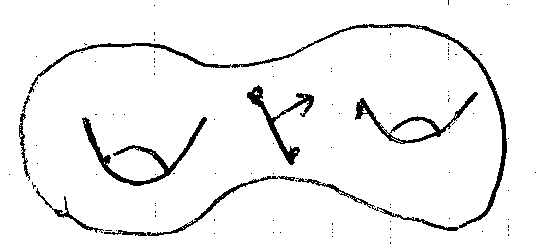
\includegraphics[width=\linewidth]{figures/gelfand-0153-p001408-hyperbolic-surface-original.png}\par\smallskip
{\footnotesize Original manuscript detail: \texttt{GELFAND-P001408}}
\end{minipage}\hfill
\begin{minipage}[t]{.50\linewidth}\vspace{0pt}\centering
{\footnotesize Partial visible-stroke recreation}\par\smallskip
\resizebox{\linewidth}{!}{% The drawn contour and interior arcs are reproduced without a genus assertion.
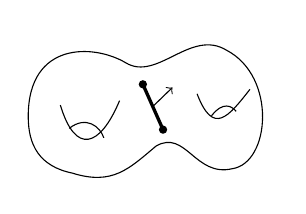
\begin{tikzpicture}[x=.8cm,y=.8cm]
\draw (0,1) .. controls (0,2.2) and (1.05,2.15) .. (1.55,1.85)
 .. controls (2.05,1.55) and (2.58,2.4) .. (3.15,2.05)
 .. controls (3.95,1.63) and (3.84,.26) .. (3.24,.17)
 .. controls (2.65,.03) and (2.5,.8) .. (2.03,.53)
 .. controls (1.6,.17) and (1.34,-.1) .. (.7,.1)
 .. controls (.17,.21) and (0,.55) .. (0,1);
\draw (.51,1.18) .. controls (.75,.38) and (1.14,.51) .. (1.45,1.25);
\draw (.65,.81) .. controls (.92,1.02) and (1.14,.84) .. (1.2,.66);
\draw (2.68,1.36) .. controls (2.94,.68) and (3.18,1.0) .. (3.52,1.43);
\draw (2.91,1.01) .. controls (3.09,1.24) and (3.23,1.17) .. (3.3,1.08);
\draw[very thick] (1.82,1.51)--(2.14,.79);
\fill (1.82,1.51) circle (1.5pt);\fill (2.14,.79) circle (1.5pt);
\draw[->] (1.97,1.15)--(2.29,1.46);
\end{tikzpicture}
}
\end{minipage}
\end{center}
\noindent{\small\textit{The outer contour, interior arcs, marked segment and branch arrow are recreated. No topology or metric is inferred from the sketch.}}
